\chapter{Methodology}\label{ch:methodology}
\section{Literature Review}
The paper \cite{gustavo_knn} proposes imputation based on K-Nearest Neighbor algorithm. They have shown that their method outperforms the internal methods used by C4.5 and CN2 to treat missing data.  It can predict both discrete attributes (the most frequent value among the k nearest neighbors) and continuous attributes(the mean among the k nearest neighbors). However the main drawback of this approach is it searches through all the data set to look for the most similar instances. It can be computationally expensive for large datasets.
\newline
In this method, the  missing  data  is  imputed  using values  from  K  most  similar  cases. For this, the k-nearest neighbors (k-nn) are selected from complete dataset. This method doesn't work for the case where there is large blocks of missing values. There will be no complete rows to perform KNN.
\newline
There exists some approaches for imputation, using neural networks. 
Wong \cite{wong_sa} suggests the imputation using sparse auto encoder. Here they have used a single layer of hidden layer. They have used their methods for missing sensor data where they exploit the spatial correlations between the data. 
\newline
In the paper \cite{collins_swarm_intelligence}, it describes a deep learning technique to extract features from the input data via an unsupervised learning approach by modeling the data distribution based on the input. This deep learning technique is then used as part of the objective function for the swarm intelligence technique in order to estimate the missing data after a supervised fine-tuning phase by minimizing an error function based on the interrelationship and correlation between features in the dataset. Here Restricted Boltzmann machines are stacked together to form an autoencoder in tandem with a swarm intelligence (SI) algorithm to estimate the missing data. This method of course has high computational time.
\newline
In paper \cite{michael_ubp}, it presents a technique for unsupervised learning called Unsupervised Backpropagation (UBP), which trains a multi-layer perceptron to fit to the manifold sampled by a set of observed point-vectors. It also assumes that there are complete data in some rows and can't solve the problem when there is not any complete data row. 
\\ 
The paper \cite{koren_netflix} uses Matrix Factorization (MF) techinque that competed in Netflix competition. MF involves factoring the data matrix into two much smaller matrices. These smaller matrices can then be combined to predict all of the missing values in the orignal dataset. It is equivalent to linear regression to project data onto its first few principal components. Unfortunately, MF is not well-suited for the data that exhibits non-linearities.
\\ Our proposed algorithm will work in non-linear data, also the extra advantage is that the trained model can be re-used in offline mode for imputation of other data from same distribution. Hence by reducing computational time for new missing datasets.
\section{Dataset Description}
The developed imputation model will be used in various real datasets as well as in synthetic datasets.
\begin{itemize}
\item \textbf{ Synthetic Datasets }
\\
The Gaussian Mixture Model (GMM) dataset will be generated and tested. This will help in understanding the type of data (based on mean, covariance) that will be supported by our proposed model. Also for training neural network , a large number of datasets is needed. Synthetic datasets will help for this as the data nature can be controlled.
\item \textbf { Real Datasets }
\\ 
Some datasets from UCI ML repository dataset \href{https://archive.ics.uci.edu/ml/datasets.html}{\textit{https://archive.ics.uci.edu/ml/datasets.html}}.
 will be used. 
 \\ Also other datasets from sensor networks \\ \href{https://github.com/karayan/FORTH_TRACE_DATASET}{\textit{https://github.com/karayan/FORTH\_TRACE\_DATASET}} will be used. This dataset is collected from 15 participants wearing 5 Shimmer sensor nodes on different parts of the body. The participants performed a series of 16 activities (7 basic and 9 postural transitions) like sitting, walking, talking, climbing etc. This dataset was used in \cite{Katerina_acm} paper for feature selection for human activity recognition. It can be assumed that a sensor node is down for few hours, resulting in block of missing values. Then it can be used as input for imputation in the proposed model.
  
\end{itemize}


\section{Deep Learning}
Deep Learning is a subfield of machine learning concerned with algorithms inspired by the structure and function of the brain called artificial neural networks.
A deep neural network (DNN) is an artificial neural network (ANN) with multiple hidden layers of units between the input and output layers. In contrary to shallow ANNs, DNNs can model complex non-linear relationships. \cite{Goodfellow_et_al_2016}. In the proposed thesis, Deep Autoencoder, consisting of multiple hidden layers is used.
\subsection{Deep Autoencoders}
An autoencoder neural network is an unsupervised learning algorithm that applies backpropagation, setting the target values to be equal to the inputs. 
i.e. \(x'_{(i)} = x_{(i)} \).
The autoencoder tries to learn a function \(h_{W,b}(x)\approx x\). In other words, it is trying to learn an approximation to the identity function, so as to output $x'$.  that is similar to $x$. The identity function seems a particularly trivial function to be trying to learn; but by placing constraints on the network, such as by limiting the number of hidden units, interesting structure about the data can be discovered. Less number of hidden neurons are placed in the middle layer than at input or output, where the data have to be projected or compressed into a lower dimensional space. \cite{hinton_autoencoder}
\\
Autoencoders also perform similar like principal component analysis (PCA) which is dimensionality reduction. While PCA performs only in linear case, autoencoder can do in non-linear data also. So, autoencoder performs good in imputation where the data lies on lower dimensional manifold. In deep autoencoder, multiple hidden layers are used.
\begin{figure}[H]
\centering
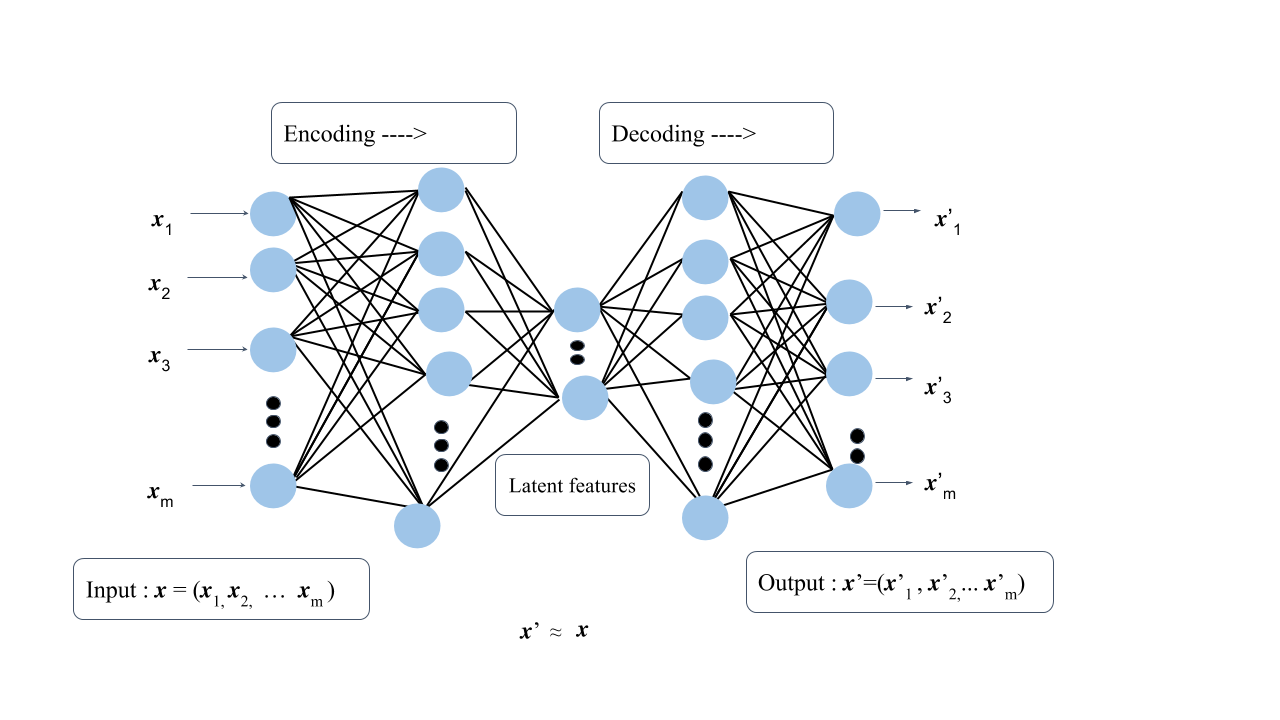
\includegraphics[width=19cm ]{figures/autoencoder.png}
\caption{\label{fig:autoencoder} Deep Autoencoder }
\end{figure}

\section{Algorithm}
For imputation with Deep Autoencoder, the forward process is same as other neural network. But caution is made during backward propagation step. During back-propagation, only the output of non missing values are used for gradient calculation. The missing input values are neglected. Some of the concepts are similar to the dropout \cite{hinton_dropout}, concept introduced by N.Srivastava, G.Hinton and his team. Here, the connection between neurons are manually dropout to reduce overfitting. In our case, the contribution of missing value inputs is made to be zero during backpropagation.
\\ Also it should be noted that not all types of dataset can be perfectly recovered. There should be some redundancy among the dataset, to have perfect reconstruction. This can be done by checking the low rank approximation of the given dataset. It indicates the existence of redundant information, giving an insight of how much accurately the data can be imputed or whether the given data is perfectly imputable or not. \cite{shabat_matrix_completion}

\begin{algorithm}
  \caption{Deep Autoencoder model training proposed algorithm for missing value imputation}\label{algorithm}
  \begin{algorithmic}[1]
	\For{ each input $x$ with incomplete data}
        \State Feed-forward pass to compute 		activations at all hidden layers, then at the output 		layer to obtain an output $x'$ 
        \State Measure the deviation of  the input         $x'$ from input $x$ as loss function
        \State Back propagate this loss function value to update weights such that only the output of non missing values is taken into consideration 
      \EndFor
      \State \textbf{result = }   Final layer output 
  \end{algorithmic}
\end{algorithm}

\section{System flow diagram}
\begin{figure}[H]
\centering
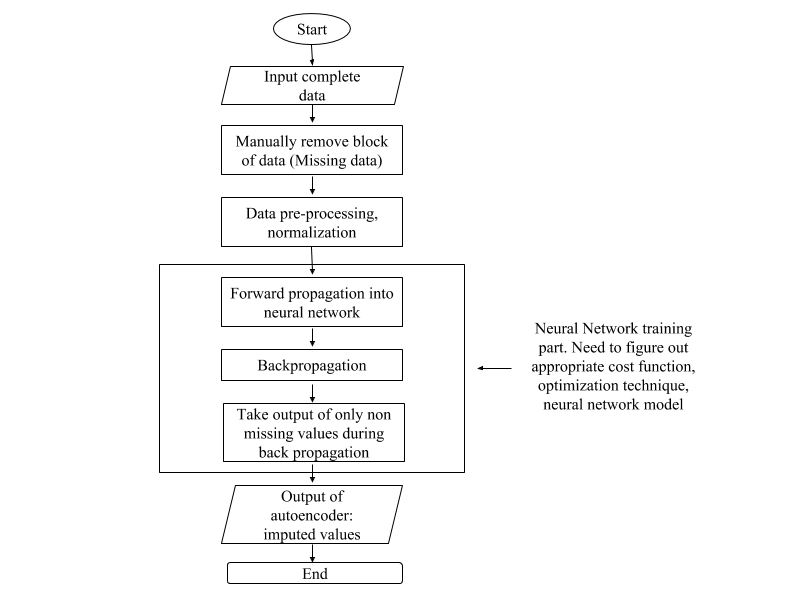
\includegraphics[width=0.99\textwidth]{figures/flowdiagram.png}
\caption{\label{fig:flowchart} System flow diagram }
\end{figure}
\vspace{3cm}
\section{ Work Plan }
\begin{enumerate}
\item Create Gaussian Mixture Model data samples with varying dimensions, mean, covariance, components
\item Implement basic Deep Autoencoder with complete dataset, to have exact output as input
\item Manually remove dataset to have missing data
\item Research on finding appropriate cost function, optimization techniques, neural network architecture to incorporate incomplete dataset
\item Test the model in various real datasets 
\end{enumerate}
\section{Tools to be used}
\begin{itemize}
\item Ubuntu Operating system (GPU supported machine will be preferred)
\item Deep learning framework: Theano or Tensorflow
\item Python programming language
\item Latex for documentation
\end{itemize}

\section{Verification and Validation}
\begin{itemize}
	\item Compare the true and imputed data samples using 	           absolute mean error
    \item Scatter plot diagram of of imputed vs non imputed
     data 
\end{itemize}








